\chapter{Theory of Constrained Optimization}
\label{chap:constrained-optimization}

\section{General Problem}

We consider the following constrained optimization problem:
\begin{equation}
    \min_{x \in \mathbb{R}^n} f(x) \quad \text{subject to} \quad
    \begin{cases}
        c_i(x) = 0, & i \in \mathcal{E}, \\
        c_i(x) \geq 0, & i \in \mathcal{I},
    \end{cases}
\end{equation}
where $f$ and $c_i$ are smooth functions, and $\mathcal{E}$ and $\mathcal{I}$ are finite index sets.

\begin{itemize}
    \item $f$: objective function.
    \item $c_i$, $i \in \mathcal{E}$: equality constraints.
    \item $c_i$, $i \in \mathcal{I}$: inequality constraints.
\end{itemize}

\section{Feasible Set}

\begin{definition}[Feasible Set]
The feasible set is the set of points that satisfy all constraints:
\begin{equation}
    \Omega = \left\{ x \in \mathbb{R}^n \mid c_i(x) = 0, \, i \in \mathcal{E} ; \; c_i(x) \geq 0, \, i \in \mathcal{I} \right\}.
\end{equation}
\end{definition}

The problem can then be equivalently written as:
\begin{equation}
    \min_{x \in \Omega} f(x).
\end{equation}

In this chapter, we will study the necessary and sufficient optimality conditions for this problem.

\section{Local Solutions}

\begin{definition}[Local Solution]
A vector $x^* \in \mathbb{R}^n$ is a \textbf{local solution} if:
\begin{enumerate}
    \item $x^* \in \Omega$, and
    \item there exists a neighborhood $\mathcal{N}$ of $x^*$ such that:
    \begin{equation}
        f(x) \geq f(x^*) \quad \text{for all } x \in \mathcal{N} \cap \Omega.
    \end{equation}
\end{enumerate}
\end{definition}

\begin{definition}[Strict Local Solution]
A vector $x^*$ is a \textbf{strict local solution} if:
\begin{enumerate}
    \item $x^* \in \Omega$, and
    \item there exists a neighborhood $\mathcal{N}$ of $x^*$ such that:
    \begin{equation}
        f(x) > f(x^*) \quad \text{for all } x \in \mathcal{N} \cap \Omega, \; x \neq x^*.
    \end{equation}
\end{enumerate}
\end{definition}

\begin{definition}[Isolated Local Solution]
A vector $x^*$ is an \textbf{isolated local solution} if:
\begin{enumerate}
    \item $x^* \in \Omega$, and
    \item there exists a neighborhood $\mathcal{N}$ of $x^*$ such that $x^*$ is the only local solution in $\mathcal{N} \cap \Omega$.
\end{enumerate}
\end{definition}

\begin{figure}[H]
\centering
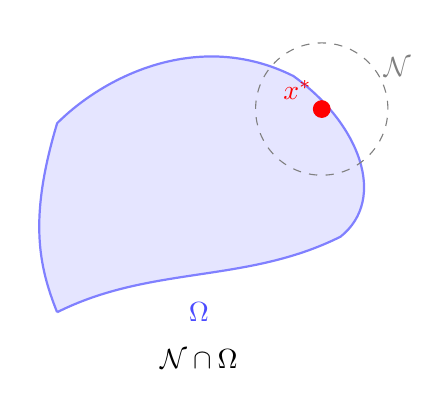
\begin{tikzpicture}[scale=1.2]
    \draw[fill=blue!10, draw=blue!50, thick] (0,0) 
        .. controls (1,0.5) and (2,0.3) .. (3,0.8)
        .. controls (3.5,1.2) and (3.2,2) .. (2.5,2.5)
        .. controls (1.5,3) and (0.5,2.5) .. (0,2)
        .. controls (-0.3,1) and (-0.2,0.5) .. (0,0);
    
    \coordinate (xstar) at (2.8, 2.15);
    \filldraw[red] (xstar) circle (2.5pt) node[above left] {$x^*$};
    
    \draw[dashed, gray] (xstar) circle (0.7cm);
    \node[gray] at (3.6, 2.6) {$\mathcal{N}$};
    
    \node[blue!70] at (1.5, 0.0) {$\Omega$};
    
    \node at (1.5, -0.5) {$\mathcal{N} \cap \Omega$};
\end{tikzpicture}
\caption{Local solution $x^*$ on the boundary of $\Omega$: the neighborhood $\mathcal{N}$ is not necessarily included in $\Omega$.}
\label{fig:local-solution-feasible}
\end{figure}

\section{Review: Smooth/Nonsmooth Problem Equivalence}

\begin{remarque}
If $g_1, \dots, g_m$ are smooth scalar functions, then the nonsmooth unconstrained problem:
\begin{equation}
    \min_{x \in \mathbb{R}^n} \left[ \max_{\mu = 1, \dots, m} g_\mu(x) \right]
\end{equation}
is equivalent to the smooth constrained problem:
\begin{equation}
    \min_{(x, t) \in \mathbb{R}^{n+1}} t \quad \text{subject to} \quad t - g_\mu(x) \geq 0, \quad \mu = 1, \dots, m.
\end{equation}
\end{remarque}

\begin{figure}[H]
\centering
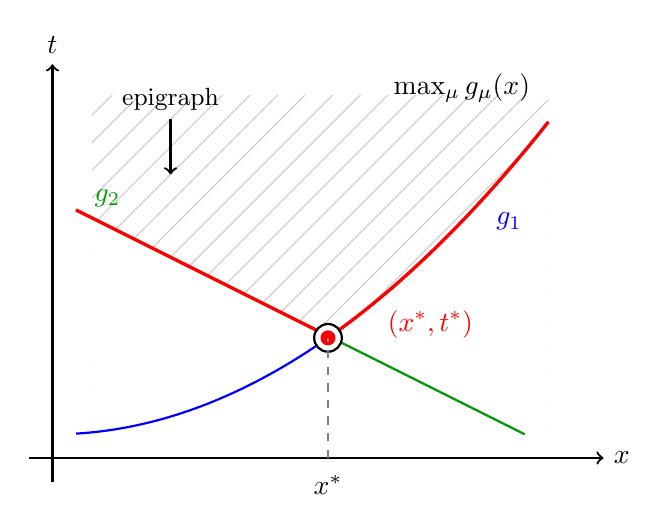
\begin{tikzpicture}[scale=1.0]
    
    % g1 = 0.1*x^2 + 0.3, g2 = -0.5*x + 3.3
    
    \begin{scope}
        \clip (0.5, 0.1) rectangle (6.3, 4.6);
        \foreach \i in {-12,-11,...,25} {
            \draw[gray!40, thin] (\i*0.35, 0) -- (\i*0.35 + 6, 6);
        }
    \end{scope}
    
    \begin{scope}
        \clip (0.5, -0.5) rectangle (3.5, 4.8);
        \fill[white] (0.5, -0.5) 
            -- plot[domain=0.5:3.5, samples=50] (\x, {-0.5*\x + 3.3})
            -- (3.5, -0.5) -- cycle;
    \end{scope}
    
    \begin{scope}
        \clip (3.5, -0.5) rectangle (6.3, 4.8);
        \fill[white] (3.5, -0.5) 
            -- (3.5, {0.1*3.5*3.5 + 0.3})
            -- plot[domain=3.5:6.3, samples=50] (\x, {0.1*\x*\x + 0.3})
            -- (6.3, -0.5) -- cycle;
    \end{scope}
    
    \draw[->, thick] (-0.3,0) -- (7,0) node[right] {$x$};
    \draw[->, thick] (0,-0.3) -- (0,5) node[above] {$t$};
    
    \draw[blue, thick, domain=0.3:6.3, samples=100] 
        plot (\x, {0.1*\x*\x + 0.3});
    \node[blue] at (5.8, 3.0) {$g_1$};
    
    \draw[green!60!black, thick, domain=0.3:6.0, samples=50] 
        plot (\x, {-0.5*\x + 3.3});
    \node[green!60!black] at (0.7, 3.3) {$g_2$};
    
    \draw[red, very thick, domain=0.3:3.5, samples=50] 
        plot (\x, {-0.5*\x + 3.3});
    \draw[red, very thick, domain=3.5:6.3, samples=50] 
        plot (\x, {0.1*\x*\x + 0.3});
    
    \coordinate (xstar) at (3.5, 1.525);
    \draw[fill=white, thick] (xstar) circle (5pt);
    \filldraw[red] (xstar) circle (2.5pt);
    
    \draw[dashed, gray] (3.5, 0) -- (3.5, 1.525);
    \node[below] at (3.5, -0.1) {$x^*$};
    
    \node[red] at (4.8, 1.7) {$(x^*, t^*)$};
    
    \node at (5.2, 4.7) {$\max_\mu g_\mu(x)$};
    
    \draw[->, thick] (1.5, 4.3) -- (1.5, 3.6);
    \node at (1.5, 4.55) {\small epigraph};
\end{tikzpicture}
\caption{Equivalence between minimizing the max (nonsmooth) and the constrained problem (smooth). The variable $t$ represents an upper bound on all functions $g_\mu$. The hatched region represents the epigraph $\{(x,t) : t \geq \max_\mu g_\mu(x)\}$. For $x < x^*$, we have $\max(g_1, g_2) = g_2$; for $x > x^*$, we have $\max(g_1, g_2) = g_1$.}
\label{fig:smooth-nonsmooth-equivalence}
\end{figure}

\begin{figureexplanation}
Figure~\ref{fig:smooth-nonsmooth-equivalence} illustrates how the problem of minimizing the maximum of several functions (red envelope, which is non-differentiable at the intersection point) can be reformulated as a smooth problem by introducing an auxiliary variable $t$ that upper bounds all functions $g_\mu(x)$. The optimal solution $(x^*, t^*)$ is located at the lowest point of the envelope, i.e., where the two functions cross.
\end{figureexplanation}

%%%%%%%%%%%%%%%%%%%%%%%%%%%%%%%%%%%%%%%%%%%%%%%%%%%%%%%%%%%%
\section{Linear Programming: The Simplex Method}
\label{sec:simplex-method}

For the special case of linear programming, we have an efficient algorithm: the simplex method.

\subsection{Standard Form}

A linear programming problem in standard form is written as:
\begin{equation}
    \min_{x \in \mathbb{R}^n} c^\top x \quad \text{s.t.} \quad Ax = b, \; x \geq 0,
\end{equation}
where $A \in \mathbb{R}^{m \times n}$, $b \in \mathbb{R}^m$, $c \in \mathbb{R}^n$.

\subsection{Basic and Nonbasic Variables}

We partition the columns of $A$ into:
\begin{itemize}
    \item $\mathcal{B}$: set of indices of the basic variables ($|\mathcal{B}| = m$).
    \item $\mathcal{N}$: set of indices of the nonbasic variables ($|\mathcal{N}| = n - m$).
\end{itemize}

We then have $B = A_{\mathcal{B}}$ (basis matrix, invertible) and $N = A_{\mathcal{N}}$.

\begin{figure}[H]
\centering
\begin{tikzpicture}[scale=1.2]
    \coordinate (A) at (0, 0);
    \coordinate (B) at (3, 0);
    \coordinate (C) at (4, 1.5);
    \coordinate (D) at (3, 3);
    \coordinate (E) at (1, 3.5);
    \coordinate (F) at (0, 2);
    
    \fill[blue!10] (A) -- (B) -- (C) -- (D) -- (E) -- (F) -- cycle;
    \draw[blue!70, thick] (A) -- (B) -- (C) -- (D) -- (E) -- (F) -- cycle;
    
    \foreach \point/\name/\pos in {A/$v_1$/below left, B/$v_2$/below right, C/$v_3$/right, D/$v_4$/above right, E/$v_5$/above, F/$v_6$/left} {
        \filldraw[red] (\point) circle (2.5pt) node[\pos] {\name};
    }
    
    \draw[->, very thick, green!60!black] (2, 1.5) -- (3.2, 2.3);
    \node[green!60!black] at (2.6, 2.6) {$\nabla c^\top x$};
    
    \draw[orange, very thick] (C) circle (5pt);
    \node[orange] at (5.8, 1.5) {\textbf{optimum} ($v_3$)};
    
    \draw[->, thick, purple] (A) -- ($(A)!0.3!(B)$);
    \draw[->, thick, purple] (B) -- ($(B)!0.3!(C)$);
    
    \node at (2, 1.2) {$\Omega$ (feasible)};
    
    \node[red, right] at (5, 3) {\small $\bullet$ Vertices = basic solutions};
    \node[purple, right] at (5, 2.5) {\small $\rightarrow$ Movement along edges};
    \node[green!60!black, right] at (5, 2) {\small Direction of decrease of $c^\top x$};
\end{tikzpicture}
\caption{Geometry of linear programming. The feasible set $\Omega$ is a polyhedron. The vertices correspond to basic feasible solutions. The simplex method moves from vertex to vertex along the edges.}
\label{fig:simplex-geometry}
\end{figure}

\begin{figureexplanation}
Figure~\ref{fig:simplex-geometry} illustrates the geometry of the linear programming problem. Basic feasible solutions correspond to the vertices of the polyhedron. The simplex method starts at a vertex and moves to an adjacent vertex that improves the objective function, until reaching the optimum (here $v_3$).
\end{figureexplanation}

\subsection{Algorithm 16: One Step of the Simplex Method}

\begin{algorithm}[H]
\caption{One step of the Simplex Method}
\label{alg:simplex}
Given $\mathcal{B}$, $\mathcal{N}$, $x_B = B^{-1}b \ge 0$, $x_N = 0$\;
Solve $B^\top\lambda = c_B$ for $\lambda$\;
Compute $s_N = c_N - N^\top\lambda$\; \Comment*[r]{Pricing}
\If{$s_N \ge 0$}{
    \Stop \Comment*[r]{optimal point found}
}
Select $q \in \mathcal{N}$ with $s_q < 0$ as the entering index\;
Solve $Bd = A_q$ for $d$\;
\If{$d \le 0$}{
    \Stop \Comment*[r]{problem is unbounded}
}
Calculate $x_q^+ = \min_{i|d_i>0}\left(\frac{(x_B)_i}{d_i}\right)$, use $p$ to denote the minimizing $i$\;
Update $x_B^+ = x_B - dx_q^+$, $x_N^+ = (0, \ldots, 0, x_q^+, 0, \ldots, 0)^\top$\;
Change $\mathcal{B}$ by adding $q$ and removing the basic variable corresponding to column $p$ of $B$\;
\end{algorithm}


%%%%%%%%%%%%%%%%%%%%%%%%%%%%%%%%%%%%%%%%%%%%%%%%%%%%%%%%%%%%
\section{Practice Exercises (Nocedal \& Wright)}
\label{sec:8.exercises}

\bigskip
\begin{exercice}[Constrained Optimization - KKT Rigor]
Consider the problem:
$$ \min_{x \in \mathbb{R}^2} f(x) = x_1 + x_2 $$
subject to the constraint $c_1(x) = x_1^2 + x_2^2 - 2 = 0$.
\begin{enumerate}
    \item Write the Lagrangian and the first-order KKT conditions.
    \item Find the candidate points $(x^*, \lambda^*)$.
    \item Verify the constraint qualification (LICQ) at these points.
    \item Verify the second-order sufficient conditions by explicitating the critical (tangent) cone $\mathcal{C}(x^*, \lambda^*)$.
\end{enumerate}
\end{exercice}

\begin{correction}
\textbf{1. KKT (First Order):}
$L(x, \lambda) = x_1 + x_2 - \lambda(x_1^2 + x_2^2 - 2)$.
Conditions (FONC):
$$ \nabla_x L = \begin{pmatrix} 1 - 2\lambda x_1 \\ 1 - 2\lambda x_2 \end{pmatrix} = 0 $$
$$ c_1(x) = x_1^2 + x_2^2 - 2 = 0 $$

\textbf{2. Candidate Points:}
$1 = 2\lambda x_1 \implies x_1 = 1/(2\lambda)$ (if $\lambda \ne 0$).
$1 = 2\lambda x_2 \implies x_2 = 1/(2\lambda)$.
Thus $x_1 = x_2$.
Constraint: $2x_1^2 = 2 \implies x_1^2 = 1 \implies x_1 = \pm 1$.
Two candidates:
- $P_1 = (1, 1)$. Then $2\lambda = 1 \implies \lambda = 1/2$.
- $P_2 = (-1, -1)$. Then $-2\lambda = 1 \implies \lambda = -1/2$.

\textbf{3. Qualification (LICQ):}
Gradient of the constraint: $\nabla c_1(x) = (2x_1, 2x_2)^\top$.
- At $P_1(1,1)$: $\nabla c_1 = (2, 2)^\top \ne 0$. Independent vectors (only 1 non-zero vector). LICQ OK.
- At $P_2(-1,-1)$: $\nabla c_1 = (-2, -2)^\top \ne 0$. LICQ OK.

\textbf{4. Second Order (SOSC):}
Hessian of the Lagrangian: $\nabla_{xx}^2 L(x, \lambda) = \nabla^2 f - \lambda \nabla^2 c_1$.
$\nabla^2 f = 0$ (linear), $\nabla^2 c_1 = \begin{pmatrix} 2 & 0 \\ 0 & 2 \end{pmatrix} = 2I$.
Thus $W = \nabla_{xx}^2 L = -2\lambda I$.

\textbf{At $P_1(1,1)$ with $\lambda = 1/2$:}
$W = -I$.
Critical cone $C(P_1) = \ker(\nabla c_1^\top) = \{ w \in \mathbb{R}^2 | (2, 2) \cdot w = 0 \} = \{ w | w_1 + w_2 = 0 \}$.
Vector in the cone: $w = (1, -1)^\top$.
Test: $w^\top W w = (1, -1) (-I) \begin{pmatrix} 1 \\ -1 \end{pmatrix} = - (1^2 + (-1)^2) = -2 < 0$.
Condition not satisfied (negative curvature). Thus $P_1$ is a local \textbf{maximum}.

\textbf{At $P_2(-1,-1)$ with $\lambda = -1/2$:}
$W = -2(-1/2)I = I$.
Critical cone $C(P_2) = \{ w | -2w_1 - 2w_2 = 0 \} = \{ w | w_1 + w_2 = 0 \}$.
Test: $w^\top W w = w^\top I w = \|w\|^2 > 0$ for all $w \ne 0$.
Sufficient condition satisfied. $P_2$ is a strict local \textbf{minimum}.
\end{correction}
\bigskip

\bigskip
\begin{exercice}[Inequalities and Critical Cone]
Consider $\min (x_1 - 1)^2 + x_2^2$ s.t. $x_1 \ge 0, x_2 \ge 0$.
Is the point $x^* = (1, 0)$ a solution?
\begin{enumerate}
    \item Verify KKT.
    \item Explicitate the critical cone $\mathcal{C}(x^*, \lambda^*)$. (Pay attention to zero/active multipliers).
    \item Verify SOSC.
\end{enumerate}
\end{exercice}

\begin{correction}
$f(x) = (x_1-1)^2 + x_2^2$. Constraints $c_1(x) = x_1 \ge 0, c_2(x) = x_2 \ge 0$.
$\nabla f = \begin{pmatrix} 2(x_1-1) \\ 2x_2 \end{pmatrix}$.
\textbf{1. KKT at $(1,0)$:}
$\nabla f(1,0) = \begin{pmatrix} 0 \\ 0 \end{pmatrix}$.
Active constraints: $c_2(x) = x_2 \ge 0$ is active ($x_2=0$). $c_1$ inactive ($x_1=1 > 0$).
Relation: $\nabla f(x^*) = \lambda_1 \nabla c_1 + \lambda_2 \nabla c_2$.
$\begin{pmatrix} 0 \\ 0 \end{pmatrix} = 0 \cdot \begin{pmatrix} 1 \\ 0 \end{pmatrix} + \lambda_2 \begin{pmatrix} 0 \\ 1 \end{pmatrix}$.
$\implies \lambda_2 = 0$. $\lambda_1=0$ (since inactive).
Multipliers are $\ge 0$. KKT satisfied.
Remark: $\lambda_2 = 0$ even though the constraint is active (degeneracy / non-strict complementarity).

\textbf{2. Critical Cone:}
$\mathcal{A}(x^*) = \{2\}$.
$C(x^*, \lambda^*) = \{ w \in \mathbb{R}^2 | \nabla c_i^\top w = 0 \text{ if } \lambda_i > 0, \text{ and } \nabla c_i^\top w \ge 0 \text{ if } \lambda_i = 0 \}$.
Here $\lambda_2 = 0$ for active constraint 2.
$\nabla c_2 = (0, 1)^\top$.
Thus conditions: $\nabla c_2^\top w \ge 0 \implies w_2 \ge 0$.
The critical cone is the upper half-plane $\{ w | w_2 \ge 0 \}$.
(This is much larger than the simple kernel $\ker \nabla c$).

\textbf{3. Second Order:}
$\nabla^2 f = \begin{pmatrix} 2 & 0 \\ 0 & 2 \end{pmatrix}$. $W = \nabla^2 f$ (since $\lambda=0$).
For any non-zero $w \in C$: $w^\top \begin{pmatrix} 2 & 0 \\ 0 & 2 \end{pmatrix} w = 2(w_1^2 + w_2^2) > 0$.
SOSC satisfied. It is a strict local minimum.
\end{correction}
\bigskip

\bigskip
\begin{checkpoint}
\begin{itemize}
    \item \textbf{Definitions:} What is an active constraint?
    \item \textbf{Qualifications:} What does LICQ mean? (Linear Independence of gradients of active constraints).
    \item \textbf{Geometry:} What is the difference between the tangent cone and the linearized cone?
\end{itemize}
\end{checkpoint}
